\chapter{Advanced Construction Algorithms for SSA
   \Author{D.~Das \andAuthor U.~Ramakrishna \andAuthor V.~Sreedhar}}
%\chapter{Alternative SSA construction algorithms
\label{chapter:alternative_ssa_construction_algorithms}
\inputpath{part1}{alternative_ssa_construction_algorithms}
\inputprogress

{

\def\p{$\phi$}
\def\st#1{\rlap{\raisebox{3.4pt}{\kern3pt{\scriptsize\it #1}}}{\rightarrow}}
\def\stplus{\rlap{\raisebox{3.4pt}{\kern3pt{\scriptsize+}}}{\rightarrow}}
\def\St#1{\rlap{\raisebox{3.4pt}{\kern3pt{\scriptsize\it #1}}}{\Rightarrow}}
\def\level{\textit{level}}

\def\p{$\phi$}
\def\iDFac{\iDF\!\!_{\textit{ac}}}


\section{Introduction}

%TODO FAB: I would prefer to remove the references to Sreedhar-Gao, Das-Ramakrishna in the main body and only refer to it in the last section. Also see if we should not completely remove the merge set.
The  placement  of $\phi$-functions is an important step in the construction of Static Single Assignment (SSA) form.
In SSA form every variable is assigned 
only once. At control-flow merge points \phifuns are added to ensure that every use of a variable corresponds to exactly one definition. 
In the rest of this chapter we will present three different approaches  for placing $\phi$-functions
at appropriate merge nodes. Recall that SSA construction falls into two phases of $\phi$-placement and variable renaming. Here we present different approaches for the first phase for minimal SSA form. We first present Sreedhar and Gao's algorithm for
placing \phifuns using the \DJ-graph\index{DJ-graph@\DJ-graph} representation of a CFG.
Then we will discuss the notions of merge set and merge relation, and present Das and Ramakrishna's algorithm for placing \phifuns based on merge relation and using \DJ-graph. Finally we describe another approach for placing \phifuns based on the loop nesting forest proposed by Ramalingam.



\section{Basic Algorithm}
The original algorithm for placing $\phi$-functions
is based on computing the dominance frontier (\DF) set for the given control-flow graph. The dominance frontier\index{dominance frontier} $\DF(x)$ of a node $x$ is the set of all nodes 
 $z$ such that $x$ dominates a predecessor of $z$, without strictly dominating $z$. Thus, from the point of view of $x$, the \DF nodes are the earliest appearance of paths joining the flow without passing through $x$.
For example, $\DF(8)= \{ 6, 8 \}$ in Figure~\ref{fig:cfg}. A straightforward algorithm for computing
\DF for each node takes $O(|V|^2)$, where $|V|$ is the number of nodes in the 
CFG, since the size of the full \DF set in the worst case can be $O(|V|^2)$.
Cytron et al.'s algorithm for the placement of $\phi$-functions consists of 
computing the iterated dominance frontier (\iDF) for a set of all definition points (or nodes where
variables are defined). 
Let $\Defs{x}$ be the set of nodes where variable $x$ are  defined.
Given that the dominance frontier for a set of nodes is just the
union of the \DF set of each node, we can compute $\iDF(\Defs{x})$ as a limit of
the following recurrence equation (where $S$ is initially $\Defs{x}$):
\begin{eqnarray*}
\iDF_1(S) &=& \DF(S) \\
\iDF_{i+1} (S) &=& \DF(S \cup \iDF_i(S)) 
\end{eqnarray*}

A $\phi$-function is then placed at each merge node in the  $\iDF(\Defs{x})$ set. 
Although Cytron et al.'s
algorithm works very well in practice, in the worst case the time complexity of $\phi$-placement algorithm for a single variable is quadratic in the number of nodes in the original control-flow graph.


\section{Placing $\phi$-functions using \DJ-graphs}
Sreedhar and Gao proposed the first linear time algorithm for computing the \iDF set without the need for explicitly computing the full \DF set. Sreedhar and Gao's original algorithm was implemented using the \DJ-graph (See Section~\ref{sec:classical_construction_algorithm:phiinsertion} and Figure~\ref{fig:classical_construction_algorithm:iDF-J}) representation of a CFG. 
The \DJ-graph for the example CFG is also shown in Figure~\ref{fig:cfg}(b). Rather than explicitly computing the \DF set, Sreedhar and Gao's algorithm uses a \DJ-graph to compute the  $\iDF(\Defs{x})$ on the fly. Even though the time complexity of Sreedhar and Gao's algorithm is linear in the size of the \DJ-graph, in practice it sometimes performs worse than the Cytron et al. algorithm. The main reason for this is that the size of the \DF set is linear in the number of nodes in the CFG 
and in practice sometimes smaller than the size of the \DJ-graph. 


\subsection{Key Observation} 
 
Now let us try to understand how to compute the \DF set for a single node using the \DJ-graph. 
Consider  the \DJ-graph shown in Figure~\ref{fig:cfg}(b). To compute $\DF(8)$ we simply walk down the
dominator (D) tree edges from node 8 and identify all join (J) edges $y \st{J} z$ such
that $z.\level \leq 8.\level$, where $\level$ of a node is the depth of the node from the
root of the dominator tree. The $\level$ of each node is also shown in Figure~\ref{fig:cfg}(b).
For our example the J edges that satisfy this 
condition are $9 \st{J} 6$ and $10 \st{J} 8$. Therefore $\DF(8) = \{6, 8\}$. To generalize the example, we can
compute the \DF of a node $x$ using:
$$\DF(x) = \{z\mid\exists\, y\in\dominated{x} \; \wedge \; y \st{J} z \in \textrm{J-edges} \; \wedge \; z.\level \leq x.\level \}$$
where 
$$\dominated{x} = \{ y\mid x\dom y \}$$


    \begin{figure}[htb]
    \centerline{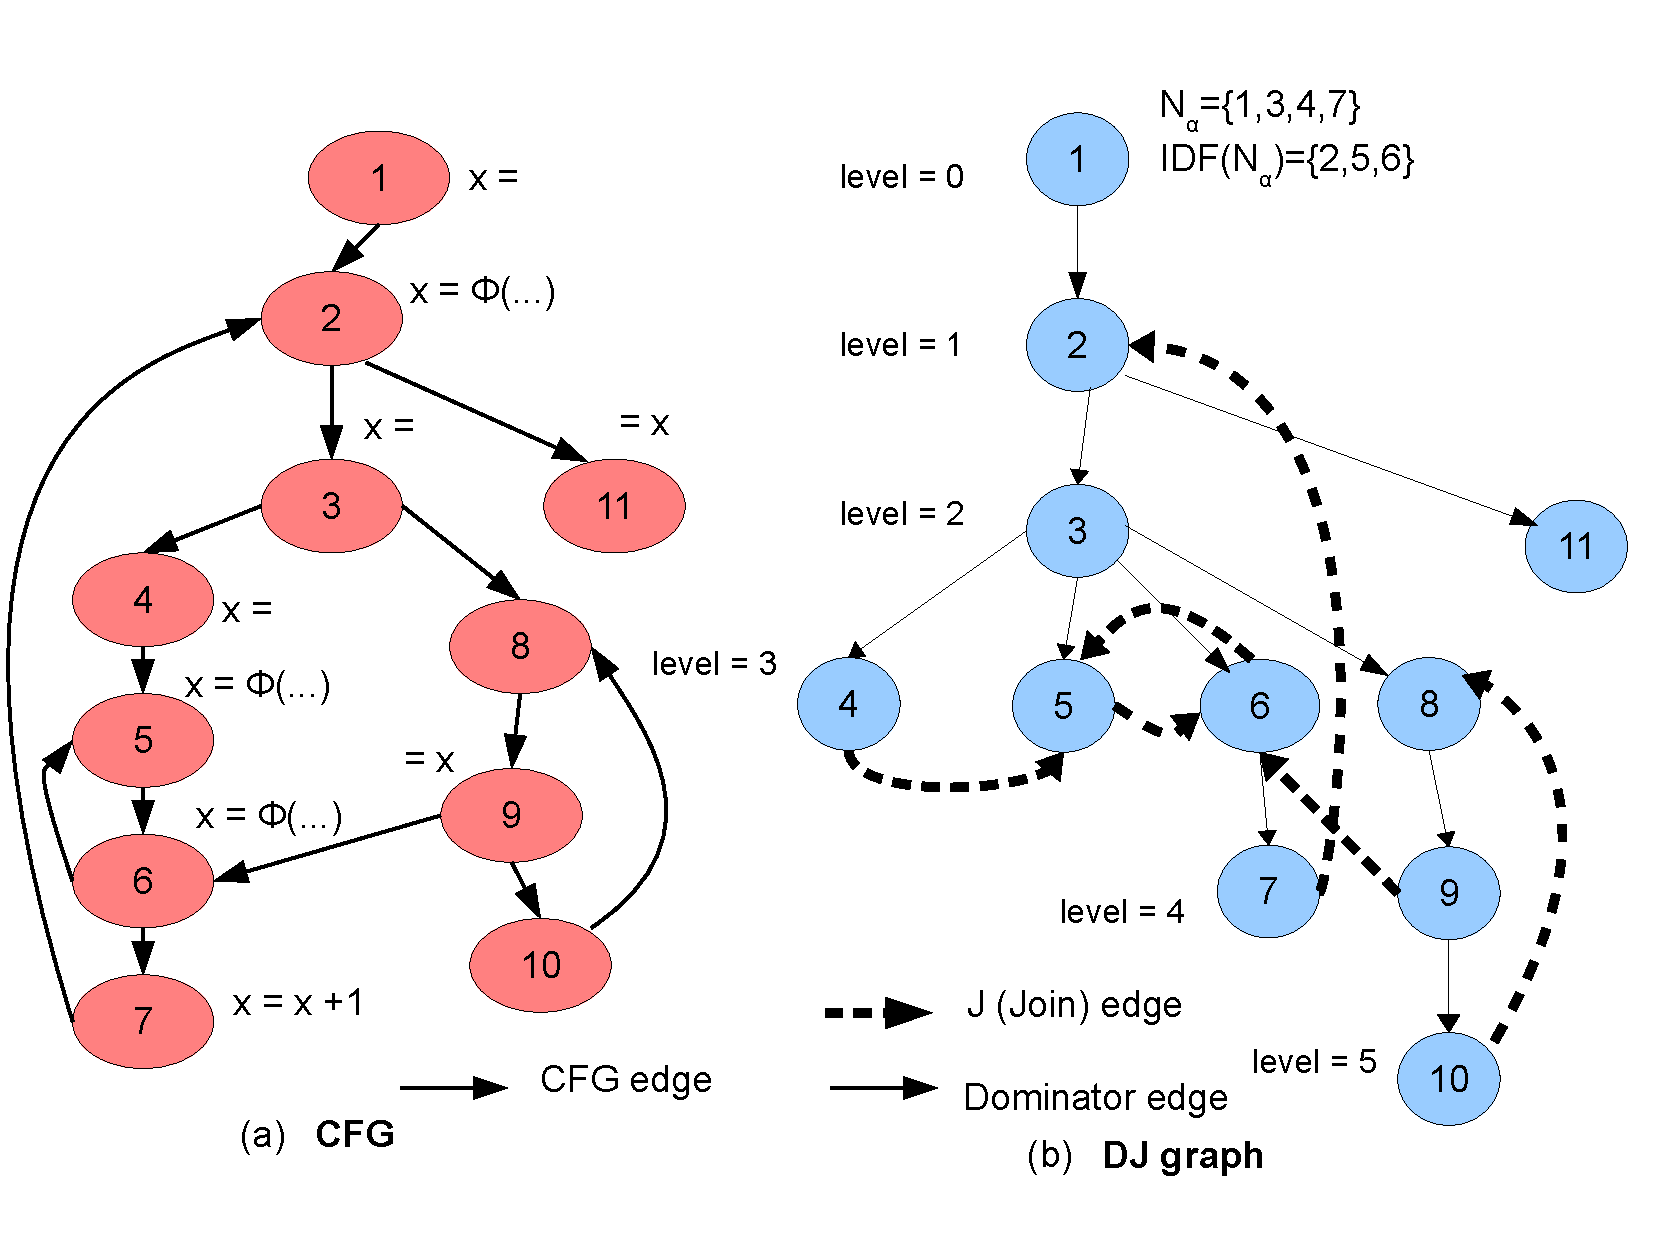
\includegraphics[scale=0.4]{cfglive_new.pdf}}
    \tikzfigure{cfglive}
    \tikzfigure{cfgdj}
    \caption{A motivating example (a) CFG (b) \DJ-graph.}
    \label{fig:cfg}
    \end{figure} 

Now we can extend the above idea to compute the \iDF for a set of nodes, and 
hence the placement of $\phi$-functions. This algorithm does not precompute \DF; given a set of initial nodes $\Defs{x}$ for which we want to compute the relevant set of $\phi$-functions,
a key observation can be made. Let $w$ be an ancestor node of a node $x$ on the dominator tree. If $\DF(x)$ has already been computed before the computation of $\DF(w)$,  the traversal of $\dominated{x}$ can be avoided and $\DF(x)$ directly used for the computation of $\DF(w)$. This is because nodes reachable from $\dominated{x}$ are already in $\DF(x)$. However, the converse may not be true, and  therefore the order of the computation of \DF is crucial.

To illustrate the key observation consider the example \DJ-graph in Figure~\ref{fig:cfg}(b),
and let us compute $\iDF(\{3,8\})$. It is clear from the recursive definition of \iDF that we have to compute $\DF(3)$ and $\DF(8)$ as a first step. Now supposing we start with node $3$ and compute $\DF(3)$. The resulting \DF set is $\DF(3) = \{2\}$. 
Now supposing we next compute the \DF set for node $8$, and the resulting set 
is $\DF(8) = \{6,8\}$. Notice here that we have already visited node $8$ and 
its subtree when visiting node $3$. We can avoid such duplicate visits by ordering the computation of \DF set so that we first compute $\DF(8)$ and then during the computation of $\DF(3)$ we avoid visiting the sub-tree of node $8$, and use the result $\DF(8)$ that was previously computed. 

Thus, to compute $\DF(x)$, where $x$ is an ancestor of $y$ in the \DJ-graph, we
do not need to compute it from scratch as we can re-use the information computed as part 
of $\DF(y)$ as shown. For this, we need to compute the \DF of deeper (based on 
level) nodes (here, $y$), before computing the \DF of a shallower node (here, 
$x$).

\begin{flalign*}
\DF(x) & = \{w \mid w \in \DF(y) \wedge w.\level \leq x.\level\} \cup \\
          &  \{w \mid t \in \textit{Subtree}(x) \setminus \textit{Subtree}(y) \wedge t \st{J} w 
          \wedge w.\level \leq x.\level \}
%}. 
\end{flalign*}

\subsection{Main Algorithm}

In this section we present Sreedhar and Gao's algorithm for computing \iDF. Let 
$x.\level$ be the
depth of the node from the root node, with $\textit{root}.\level= 0$. To ensure that the 
nodes are processed according to the key observation we use  a simple array of 
sets \textit{OrderedBucket}, and two functions defined over this array of sets:
(1) InsertNode($n$) that inserts the node $n$ in the set 
$\textit{OrderedBucket}[n.\level]$, and
(2) GetDeepestNode() that returns a node from the \textit{OrderedBucket} with the deepest level number. 

\begin{algorithm}
  \caption{Sreedhar and Gao's algorithm for computing \iDF set.}
  \label{algo:IDFMain}

  \KwIn{\DJ-graph representation of a program}
  \KwIn{$\Defs{x}$: nodes that define $x$}
  \KwOut{$\iDF(\Defs{x})$}

  $\iDF \gets \emptyset$\;
  \ForEach{node $x \in  \mbox{\Defs{x}}$}{
    InsertNode($x$)\;
    $x.\textit{visited} \gets \false $\;
  }
  \While(\tcc*[f]{Get node from the deepest level}){$z \gets \textit{GetDeepestNode}()$}{  \label{C:get} 
    $\textit{currentRoot} \gets z$\;
    $z.\textit{visited} \gets \true$\;
    Visit($z$)\tcc*[r]{Find $\DF(z)$}
  }
\end{algorithm}


\begin{procedure}
  \caption{Visit(x)}
  \label{proc:visit}
  \ForEach{node $y \in \textit{Succ}(x)$}{
    \If{$x \st{} y$ is a  J edge}{
      \If{$y.\level \leq \textit{currentRoot}.\level$}{
        \If{$y \not \in \iDF$}{
          $\iDF \gets \iDF \cup {y}$\;   \label{C:idf}
          \lIf{$y \not  \in \Defs{x}$}{
            InsertNode($y$); \label{C:insert}
          }
        }
      }
    }
    \Else(\tcc*[f]{visit D edges}){
    \If{$y.\textit{visited} = \false $}{
      $y.\textit{visited} \gets \true$\;
      \tcc{if($y.\textit{boundary} = \false$)   \label{C:cached} // See the section on Further Reading for details}
      Visit($y$)\; \label{C:dedges}
      }
    }
  }
\end{procedure}

In Algorithm~\ref{algo:IDFMain}, at first we insert all nodes belonging to $\Defs{x}$ in the 
\textit{OrderedBucket}. Then the nodes are processed
in a bottom-up fashion over the \DJ-graph from deepest node level to least node level
by calling \ref{proc:visit}($x$). The procedure \ref{proc:visit}($x$) essentially 
walks top-down in the  \DJ-graph avoiding already visited nodes. During this 
traversal it also peeks at destination nodes of J edges. Whenever it notices 
that the level number of the destination node of a J edge is less than or equal 
to the level number of the $\textit{currentRoot}$, the destination node is 
added to the $\iDF$ set (Line~\ref{C:idf}) if it is not present in \iDF already. 
Notice that at Line~\ref{C:insert} the destination node is also inserted in the 
{\it OrderedBucket} if it was never inserted before. Finally at Line 
\ref{C:dedges} we continue to process the nodes in the sub-tree by visiting 
over the D edges. When the algorithm terminates the 
set $\iDF$ contains the iterated dominance frontier for the initial $\Defs{x}$.

    \begin{figure}[htb]
    \centerline{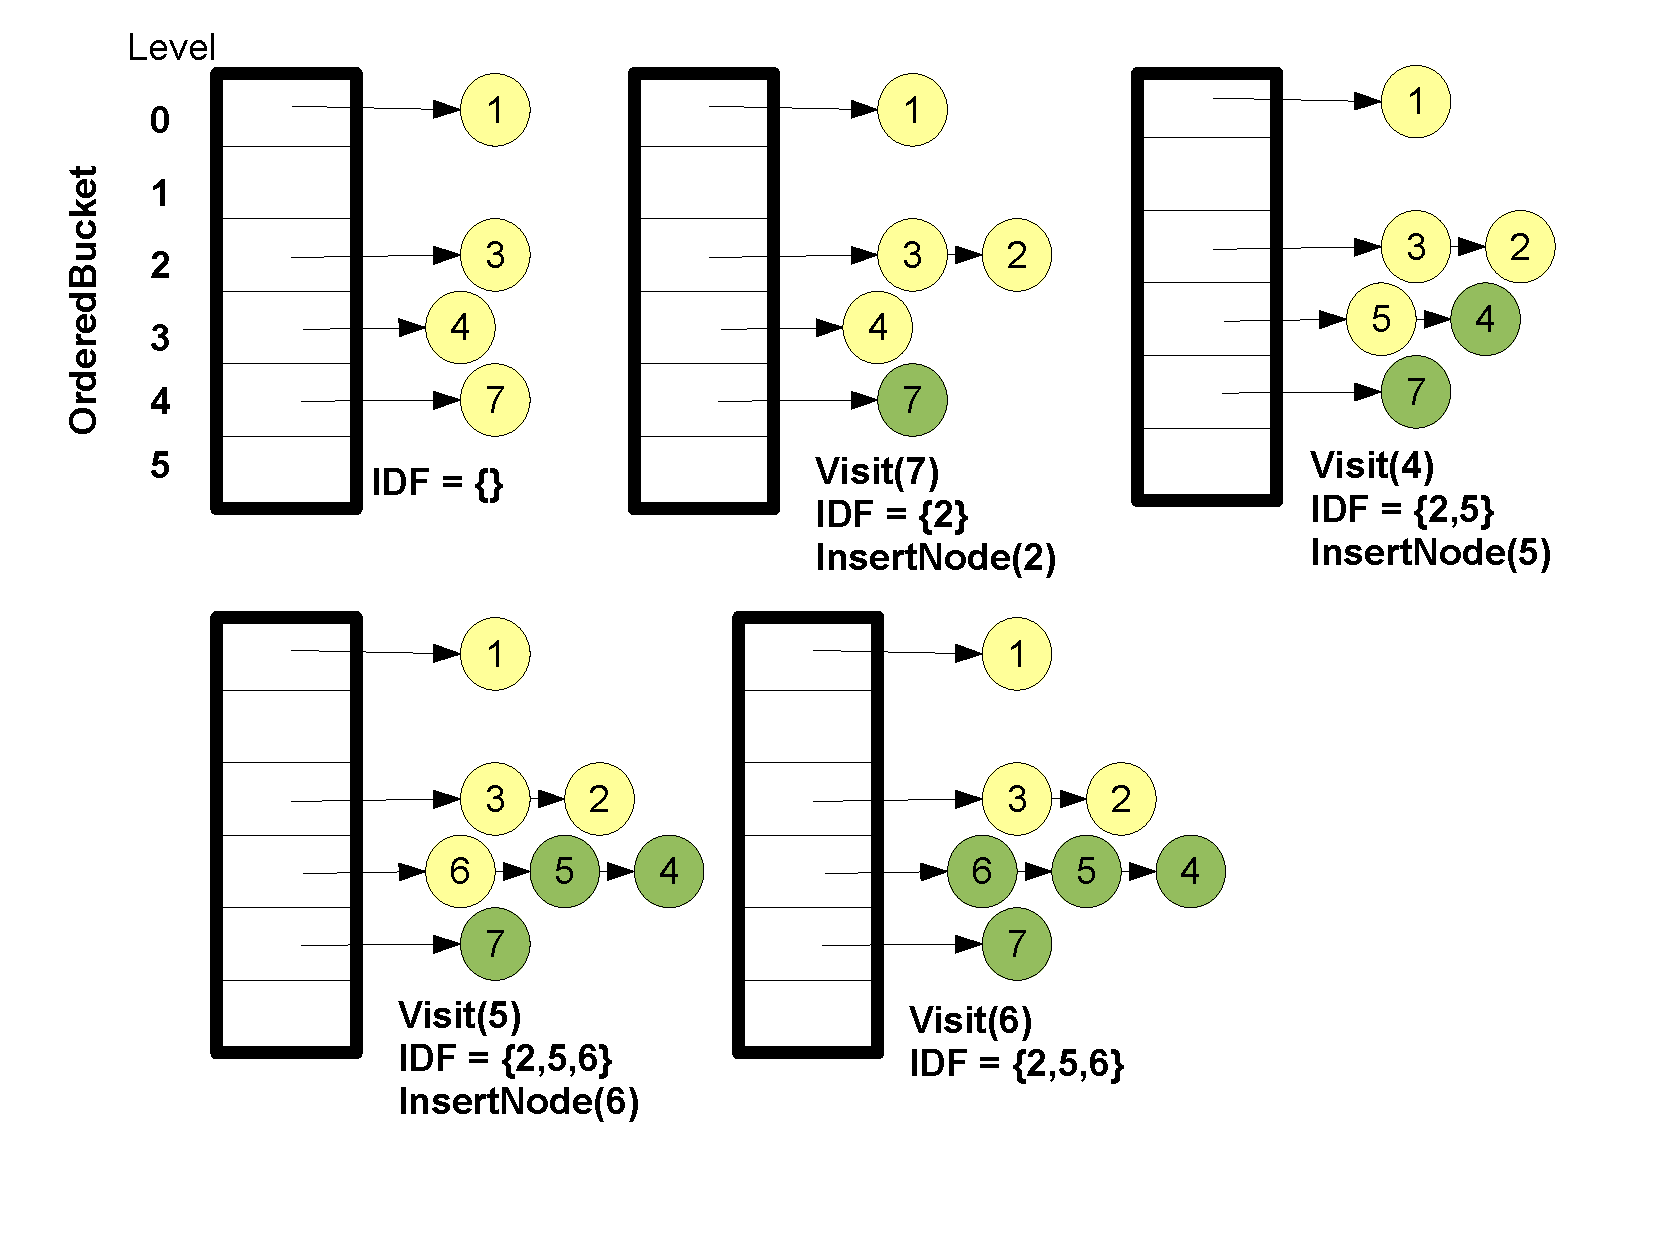
\includegraphics[scale=0.3]{sreedhargao.pdf}}
    \caption{Phases of Sreedhar and Gao's algorithm for $\Defs{x}=\{1,3,4,7\}$.}
    \label{fig:sreedhargao}
    \end{figure} 


In Figure~\ref{fig:sreedhargao}, some of the phases of the algorithm are 
depicted for clarity. The \textit{OrderedBucket}
is populated with the nodes $1,3,4$ and $7$ corresponding to $\Defs{x}=\{1,3,4,7\}$. The nodes are
placed in the buckets corresponding to the levels at which they appear. Hence, node 1 which appears at 
level 0 is in the zero-th bucket, node 3 is in the second bucket and so on. Since the
nodes are processed bottom-up, the first node that is visited is node 7. The successor of node 7 is node
2 and since there exists a J edge $7 \st{J} 2$, and the $\iDF$ set is empty, the $\iDF$ set is updated
to hold node~2 according to Line~\ref{C:idf} of the \texttt{Visit} procedure. In addition, InsertNode(2) is invoked and 
node~2 is placed in the second bucket. The next node visited is node~4. The successor of node~4 which is node
5 has an incoming J edge $4 \st{J} 5$ which results in the new $\iDF = \{2,5\}$. The final $\iDF$ set converges
to $\{2,5,6\}$ when node~5 is visited. Subsequent visits of other nodes do not add anything to the
$\iDF$ set. An interesting case arises when node 3 is visited. Node 3 finally causes nodes 9 and 10 also 
to be visited. However, when node 10 is visited, its successor node which is node 8 and which also 
corresponds to the J edge $10 \st{J} 8$, does not result in an update of the $\iDF$ set as the level of
node~8 is deeper than that of node~3.


\section{Placing $\phi$-functions using Merge Sets}

In the previous section we described $\phi$-function placement algorithm in terms of iterated dominance frontiers. There is another way to approach the problem
of \phifun placement using the concepts of merge relation and merge set. In this section
we will first introduce the notion of merge set and merge relation and then show
how the merge relation is related to the \DF relation. We will then show how to compute
the M (merge) graph\index{merge graph} using the \DJ-graph and then use the M-graph for placing $\phi$-functions.

\subsection{Merge Set and Merge Relation}

First, let us define the notion of a {\em join} set $J(S)$
 for a given set of nodes  $S$ in a control-flow graph.\footnote{In English, ``join'' and ``merge'' are synonyms, 
but unfortunately
in the literature, due to lack of  better terms, these two synonyms are used to mean
distinct but related concepts.} Consider two nodes $u$ and $v$ and distinct 
non-empty (denoted by +)
paths from $u \stplus w$ and $v \stplus w$, where $w$ is some node in the CFG. If the 
two paths meet only at $w$ then $w$ is in the join set of the nodes $\{u, v\}$. 
For instance, consider nodes 1 and 9 in Figure~\ref{fig:cfg}(a).
The paths $1 \st{} 2 \st{} 3 \st{} 8$ and $9 \st{} 10 \st{} 8$ meet at $8$ 
for the first time and so $\{8\} \in J(\{1,9\})$. 

Now let us define the {\em merge} relation as a relation 
$v=M(u)$ that holds between two nodes $u$ and $v$ whenever
$v \in J(\{\textit{root}, u\})$. We insert a $\phi$-function at $v$ for a variable that is assigned
only at $\textit{root}$ and $u$. One can show that $J(S) = \cup_{u \in S} M(u)$ where $S \subseteq V$. Also, for any node $u \in V$, $v \in M(u)$ if and only if
there is a path $u \stplus v$ that does not contain $\textit{idom}(v)$.  This relationship between
dominance and merge can be conveniently encoded using a \DJ-graph and can be used for placing 
$\phi$-functions. First, we will construct the \DF (Dominance Frontier) graph using the \DJ-graph. For each J edge $u \st{} v$ in the \DJ-graph insert a new  $w \st{J} v$ where
$w = \textit{idom} (u)$ and $w$ does not strictly dominate $v$. Another way to look at 
this is to insert a new J edge $w \st{} v$ if $w = \textit{idom}(u)$ and $w.\level \geq 
v.\level$.\footnote{Recall that $w.\level$ is the depth of $w$ from the
$\textit{root}$ of the dominator tree.} We repeatedly insert new J edges in a bottom-up fashion over the \DJ-graph until no more J edge can be inserted. The resulting \DJ-graph is a ``fully cached'' \DJ-graph. We will call the fully cached DJ-graph the \DF-graph.

Next, we can compute the M relation from the \DF-graph. 
Using the \DF-graph we compute the M-graph as a transitive closure
using only the \DF edges of the \DJ-graph. In Figure~\ref{fig:mgraph}, $M(4) = 
\{2,5,6\}$ as the nodes 2, 5 and 6 are the only nodes reachable from node~4 
following the \DF edges. Similarly, for node~8, $M(8) = \{2,5,6,8\}$ due to these nodes being reachable from node 8 via the \DF edges. Given the M-graph of a CFG we can place $\phi$-functions for a set $S \subseteq V$ at $M(S)$.

    \begin{figure}[htb]
    \centerline{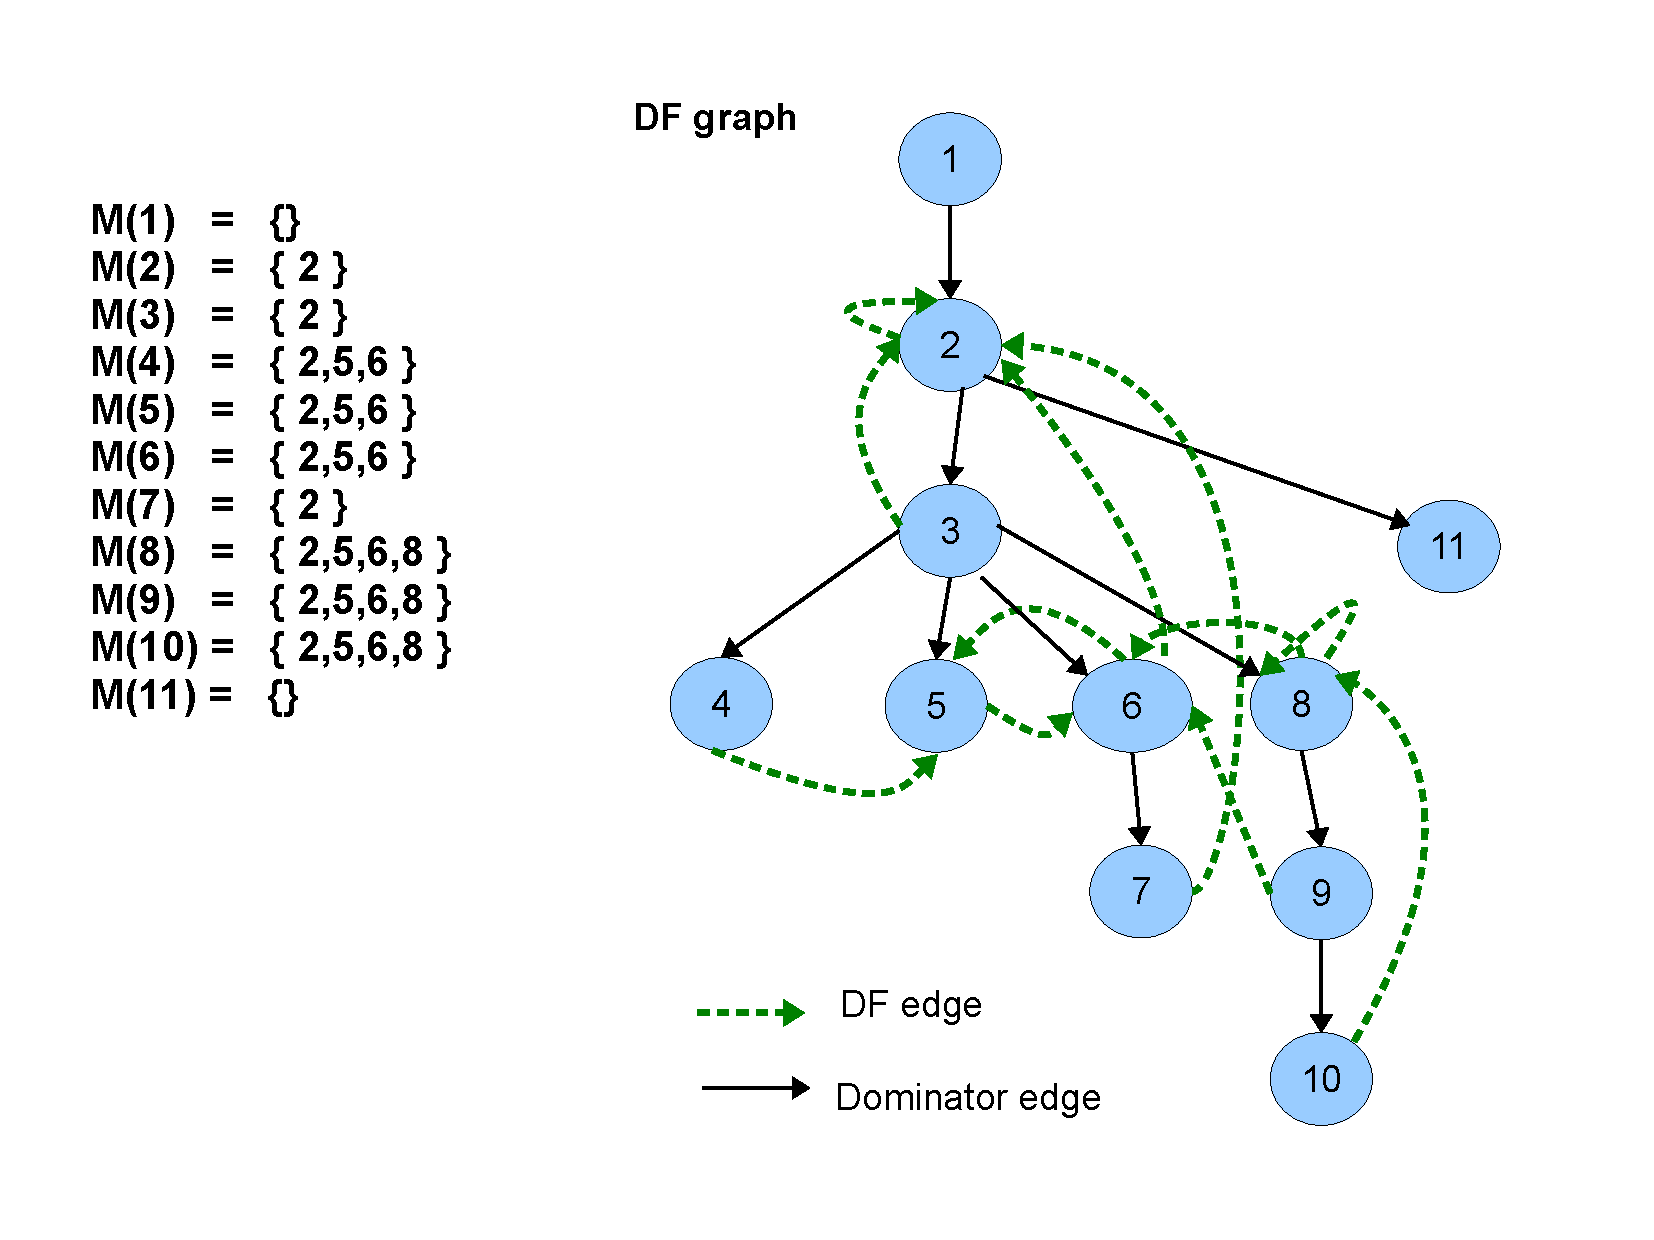
\includegraphics[scale=0.4]{mgraph_1.pdf}}
    \caption{\DF-graph and M sets.}
    \label{fig:mgraph}
    \end{figure} 


The algorithms for placing $\phi$-functions based on the construction of the 
\DF-graph or M relation can be quadratic in the worst case. The merge relation 
is due to Pingali and Bilardi. The \DF-graph and the M sets for the running 
example are given in Figure~\ref{fig:mgraph}.

\subsection{Iterative Merge Set Computation}
In this section we describe a method to iteratively compute the 
$\textit{merge}$ relation using a data-flow formulation. In the previous section 
we saw that the $\textit{merge}$ relation can be computed using a transitive 
closure of the \DF-graph, which in turn can be computed from the \DJ-graph. In 
the algorithm proposed by Das and Ramakrishna, explicit \DF-graph construction 
or the transitive closure formation are not necessary. Instead, the same result 
can be achieved by formulating the $\textit{merge}$ relation as a data-flow 
problem and solving it iteratively. For several applications, this approach has 
been found to be a fast and effective method to construct $M(x)$ for each node 
$x$ and the corresponding $\phi$-function placement using the $M(x)$ sets. 

Consider a J edge $u \st{J} v$. Also consider all nodes $w$ such that $w$ 
dominates $u$ and $w.\level \geq v.\level$. For every $w$ we can set up the 
data-flow equation as $M(w) = M(w) \cup M(v) \cup \{v\}$. The set of data-flow 
equations for each node $n$ in the \DJ-graph can be solved iteratively using a 
top-down pass over the \DJ-graph. To check whether multiple-passes are required 
over the \DJ-graph before a fixed-point is reached for the data-flow equations, 
we devise an ``inconsistency condition'' stated as follows:

%\paragraph{Inconsistency Condition:}
\begin{center}
\bf{Inconsistency Condition:}\\
\it{For a J edge, $u \st{J} v$, if $u$ does not satisfy
$M(u)\supseteq M(v)$,\\ then the node $u$ is said to be inconsistent}. 
\end{center}

The algorithm described in the next section is directly based on the method of building
up the $M(x)$ sets of the nodes as each J edge is encountered in an iterative fashion by
traversing the \DJ-graph top-down. If no node is found to be \emph{inconsistent} after a single 
top-down pass, all the nodes are supposed to have reached fixed-point solutions. If some node
is found to be inconsistent, multiple passes are required until a fixed-point solution is reached.


\subsubsection{Top Down Merge Set Computation}

%==
\begin{figure}[!ht]
\centering
\begin{minipage}[t]{5in}
\noindent{\bf Input:} A \DJ-graph representation of a program.
\noindent{\bf Output:} The merge sets for the nodes.

\setcounter{linectr}{0}
Procedure TDMSCMain
\{
\begin{code}
\x1 $\forall$ node $x \in$ \DJ-graph set $M(x) = \{\}$
\x1 {\it done = false};
\x1 {\bf while} (! {\it done}) {\bf do}
\x2     {\it done} = TDMSC-I(\DJ-graph);
\x1 {\bf end while}
\end{code}
\}

Procedure TDMSC-I(\DJ-graph)
\{
\begin{code}
%\textbf{Algorithm: Top Down Merge Set Computation (TDMSC-I)}
%Input: $\DJ$-graph
%Outputs: Complete Merge Sets for every node of the \DJ-graph

\x1 $\textit{RequireAnotherPass}=\false$;

\x1 {\bf while} (n = next node in B(readth) F(irst) S(earch) order of \DJ-graph) {\bf do} \label{C:bfs}
%\x2      $n$ $=$ Next Node in BFS list
\x2      {\bf for} ($\forall$ incoming edge to $n$) {\bf do} \label{C:jedge}

\x3          Let $e = s \st{J} n$ , be an incoming J edge
\x3          {\bf if} ($e$ not visited) {\bf then}
\x4              Mark $e$ as visited 
\x4              $\textit{tmp}$ $=$ $s$;
\x4              $\textit{lnode}$ $=$ $\nullprog$;
\x4              {\bf while} $(\level(tmp)\ge \level(n))$ {\bf do} \label{C:mwhiles}

\x5                   $M(tmp)=M(tmp)\cup M(n)\cup \{n\}$;
\x5                   $lnode=tmp$;
\x5                   $tmp=parent(tmp)$; //dominator tree parent
\x4              {\bf end while} \label{C:mwhilee}
\x4              {\bf for} ($\forall$ incoming edge to $lnode$) {\bf do} \label{C:lnode}
\x5                  Let $e'$ $=$ $s^{'} \st{J} lnode$, be an incoming J edge
\x5                  {\bf if} ($e'$ visited) {\bf then}
\x6                     {\bf if} $(M(s') \not\supseteq M(lnode))$ {\bf then} //Check inconsistency
\x7                         $RequireAnotherPass = true$;
\x6                     {\bf end if}
\x5                  {\bf end if}
\x4              {\bf end for}
\x3          {\bf end if}
\x2     {\bf end for}
\x1 {\bf end while}
\x1 {\bf return} $RequireAnotherPass$;
\end{code}
\}
\end{minipage}
\caption{Top Down Merge Set Computation algorithm for computing Merge sets.}
\label{F:tdmsc}
\end{figure} 

The first and direct variant of the approach laid out above is poetically 
termed TDMSC-I. This variant works by scanning the \DJ-graph in a top-down 
fashion as shown in Line~\ref{C:bfs} of Figure~\ref{F:tdmsc}. All $M(x)$ sets 
are set to the empty set before the initial pass of TDMSC-I. The $M(x)$ sets 
computed in a previous pass are carried over if a subsequent pass is required. 

The \DJ-graph is visited
level by level. During this process, for each node $n$ encountered, if there is 
an \emph{incoming}
J edge $s \st{J} n$ as in Line~\ref{C:jedge}, then a separate bottom-up pass starts at 
Line~\ref{C:mwhiles}. This bottom-up pass traverses all nodes $w$ such that $w$ 
dominates $s$ and $w.\level \geq s.\level$,
updating the $M(w)$ values using the aforementioned data-flow equation. Line~\ref{C:lnode} is used for
the inconsistency check. \textit{RequireAnotherPass} is set to true only if a fixed point is not reached
and the inconsistency check succeeds for some node.

There are some subtleties in the algorithm that should be noted. 
Line~\ref{C:lnode} of the algorithm visits incoming edges to \textit{lnode} 
only when \textit{lnode} is at the same level as $n$, which is the current 
level of inspection and the incoming edges to \textit{lnode}'s posterity are at 
a level greater than that of node $n$ and are unvisited yet. 

Here, we will briefly walk through TDMSC-I using the \DJ-graph of Figure~\ref{fig:cfg}(b). Moving top-down over the graph, the first J edge encountered is $7 \st{J} 2$. As a result, a bottom-up climbing of the nodes happens, starting at node $7$ and
ending at node $2$ and the merge sets of these nodes are updated so that $M(7) = M(6) = M(3) = M(2) = \{2\}$. The next J edge
to be visited can be any of $4 \st{J} 5$, $5 \st{J} 6$ or $6 \st{J} 5$ at 
$\level = 3$. Assume it is $5 \st{J} 6$. This results in $M(5) = M(5) \cup M(6) 
\cup \{6\} = \{2,6\}$. Now, let $6 \st{J} 5$ be visited. Hence, $M(6) = M(6) 
\cup M(5) \cup \{5\} = \{2,5,6\}$. At this point, the \emph{inconsistency check} 
comes into picture for the edge $6 \st{J} 5$, as $5 \st{J} 6$ is another J edge 
that is already visited and is an incoming edge of node $6$. Checking for $M(5) 
\supseteq M(6)$ fails, implying that the $M(5)$ needs to be computed again. 
This will be done in a succeeding pass as suggested by the 
\textit{RequireAnotherPass} value of true. In a second iterative pass, the J edges are visited in the same order. Now, when $5 \st{J} 6$ is visited, 
$M(5) = M(5) \cup M(6) \cup \{6\} = \{2,5,6\}$ as this time 
$M(5) = \{2,6\}$ 
and $M(6) = \{2,5,6\}$. On a subsequent visit of $6 \st{J} 5$, $M(6)$ is also set to $\{2,5,6\}$. The inconsistency does not appear any more and the algorithm proceeds to handle the edges $4 \st{J} 5$, $9 \st{J} 6$ and $10 \st{J} 8$ which have
also been visited in the earlier pass. TDMSC-I is invoked repeatedly by a different function
which calls it in a loop till \textit{RequireAnotherPass} is returned as \false as shown in the procedure TDMSCMain.

%\subsubsection { Final $\phi$-function placement using Merge Sets }
Once the $Merge$ relation is computed for the entire CFG, placing $\phi$ is a straightforward application of the $M(x)$ values for a given $\Defs{x}$, as shown in Figure~\ref{F:phip}.
\begin{figure}[!ht]
\centering
\begin{minipage}[t]{5in}
\noindent{\bf Input:} A CFG with Merge sets computed and $\Defs{x}$.
\noindent{\bf Output:} Blocks augmented by $\phi$-functions for the given $\Defs{x}$.

\setcounter{linectr}{0}

Procedure $\phi$-placement for $\Defs{x}$
\{
\begin{code}
\x1 {\bf for} ($\forall n \in \Defs{x}$) {\bf do}
\x2   {\bf for} ($\forall n^{'} \in M(n)$) {\bf do}
\x3       Add a $\phi$ for $n$ in $n^{'}$ if not placed already
\x2   {\bf end for}
\x1 {\bf end for}
\end{code}
\}
\end{minipage}
\caption{$\phi$-placement using $Merge$ sets.}
\label{F:phip}
\end{figure} 


\section{Computing Iterated Dominance Frontier Using Loop Nesting Forests}
\label{section:alternative_ssa_construction_algorithms:loop}
This section illustrates the use of \emph{loop nesting forests} to construct 
the iterated dominance frontier (\iDF) of a set of vertices in a CFG. This 
method works with reducible as well as irreducible loops and is based on 
Ramalingam's work.


\subsection{Loop nesting forest}
\index{loop nesting forest}
A loop nesting forest is a data structure that represents the loops in a CFG 
and the containment relation between them. In the example shown in 
Figure~\ref{fig:lnf}(a) the loops with back edges $11 \rightarrow 9$ and $12 \rightarrow 2$ are both reducible loops. The corresponding loop nesting forest is shown in Figure~\ref{fig:lnf}(b) and consists of two loops whose header nodes are $2$ and $9$. The loop with header node $2$ contains the loop with header node $9$.

    \begin{figure}[htb]
    \centerline{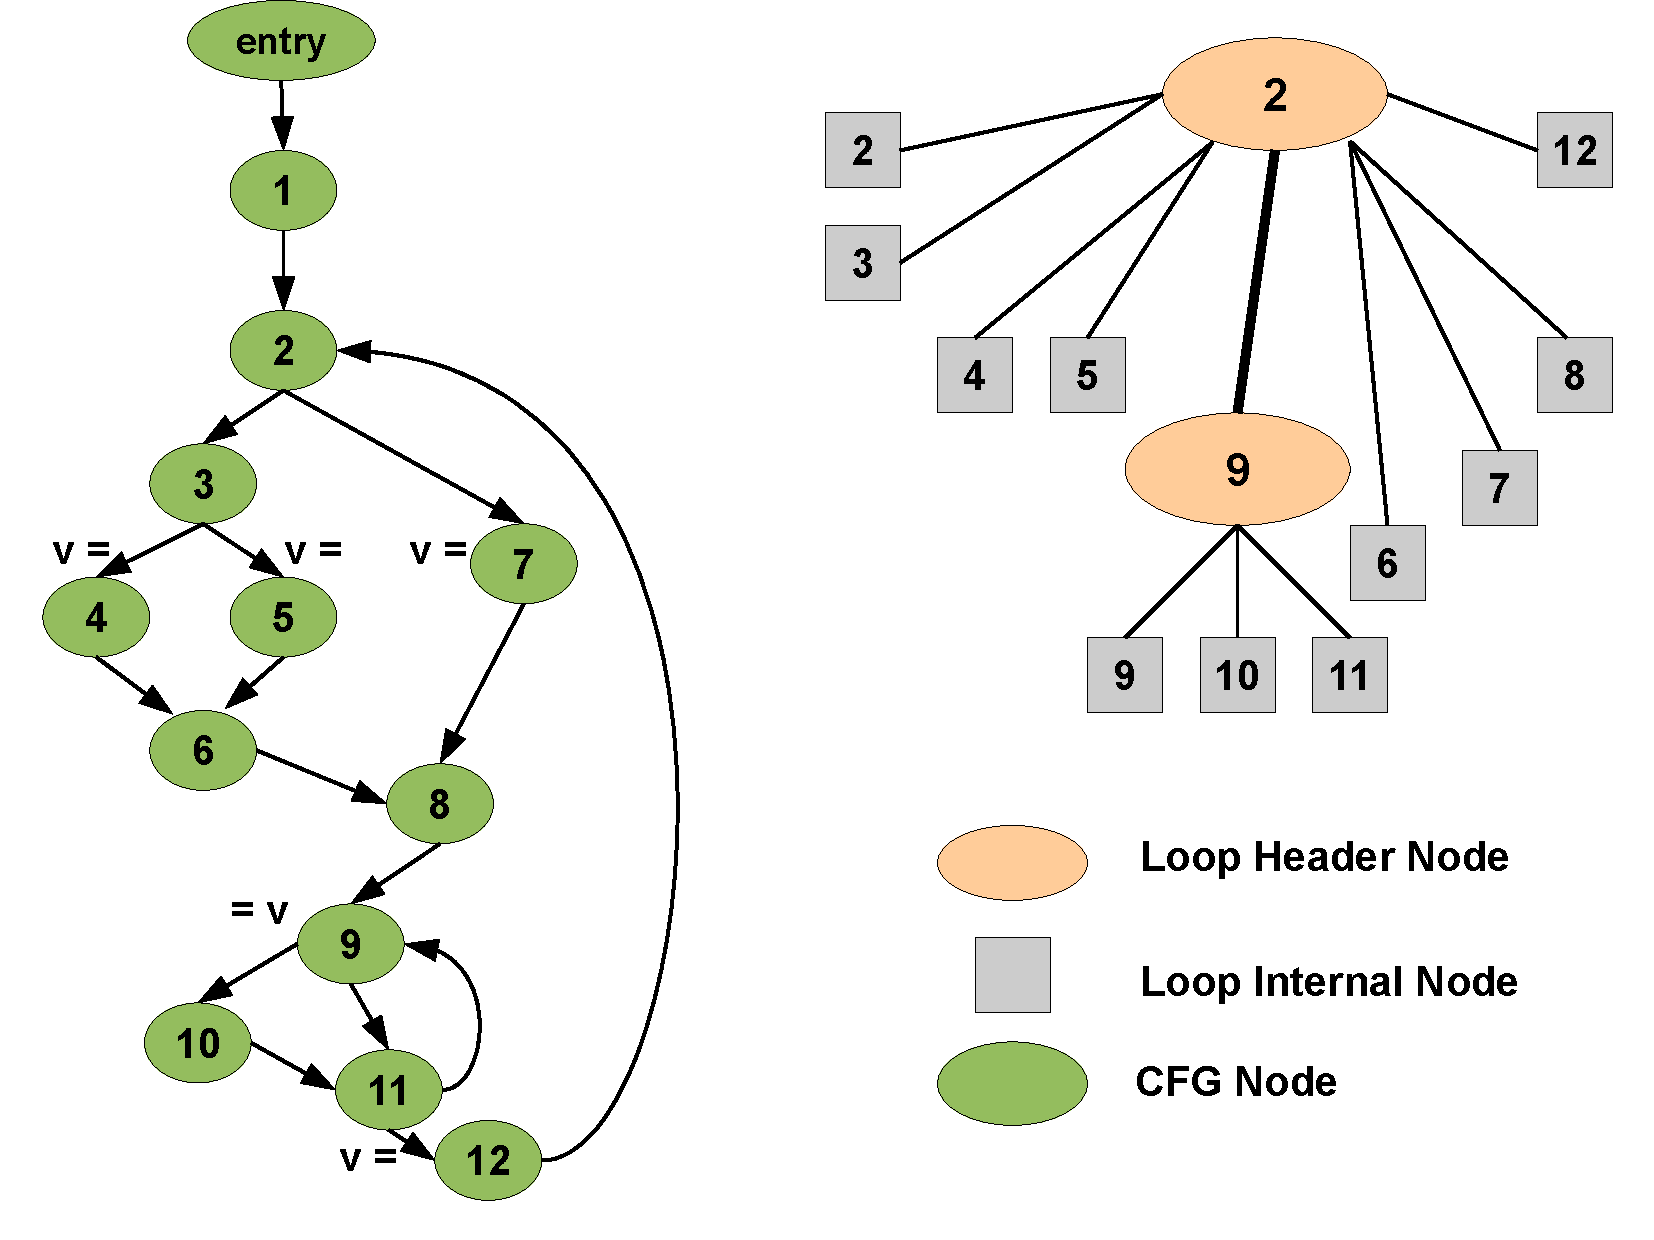
\includegraphics[scale=0.3]{lnfred.pdf}}
    \caption{An example (a) CFG and (b) Loop Nesting Forest.}
    \label{fig:lnf}
    \end{figure} 


\subsection{Main Algorithm}

The idea is to use an acyclic version of the control-flow graph (i.e., without 
back edge) and construct the \iDF for a variable in this context: whenever two 
definitions reach a join point, it belongs to the \iDF. Then, we take into 
account the back edges using the loop nesting forest: if a loop contains a 
definition, its header also belongs to the \iDF.

\medskip
    
A definition node $d$ ``reaches'' another node $u$ if there is a path in the 
graph from $d$ to $u$ which does not contain any re-definition. If at least two 
definitions reach a node $u$, then $u$ belongs to $\iDF(X)$ where $X$ consists 
of these definition nodes. This suggests the Algorithm~\ref{algo:ramaIDF} which 
works for \emph{acyclic} graphs.
For a given $\Defs{x}$, we can compute $\iDF(\Defs{x})$ as follows:

\begin{itemize}
\item { Initialize \iDF to the empty set };
\item { Using a topological order, compute the subset of $\iDF(\Defs{x})$ that can reach a node using forward data-flow analysis };
{\item} {Add a node to \iDF if it is reachable from multiple nodes};
\end{itemize}  

For Figure~\ref{fig:lnf}, the acyclic version of the graph $G$, termed 
$G_{\textit{ac}}$, is formed by dropping the back edges $11 \rightarrow 9$ and $12 
\rightarrow 2$. Also, $\textit{entry}(G) = \{\textit{entry}\}$ where 
$\textit{entry}$ is a specially designated node that is the root of the 
CFG. For the definitions of $v$ in nodes $4,5,7$ and $12$ in 
Figure~\ref{fig:lnf}, the subsequent nodes reached by multiple definitions 
are $6$ and $8$: node $6$ can be reached by any one of two definitions in 
nodes $4$ or $5$, and node $8$ by either the definition from node 
$7$ or one of $4$ or $5$. Note that the back edges do not exist in the 
acyclic graph and hence node~$2$ is not part of the \iDF set. We will see 
later how the \iDF set for the entire graph is computed by considering the 
contribution of the back edges. 



%\begin{figure}[htb]
%\centerline{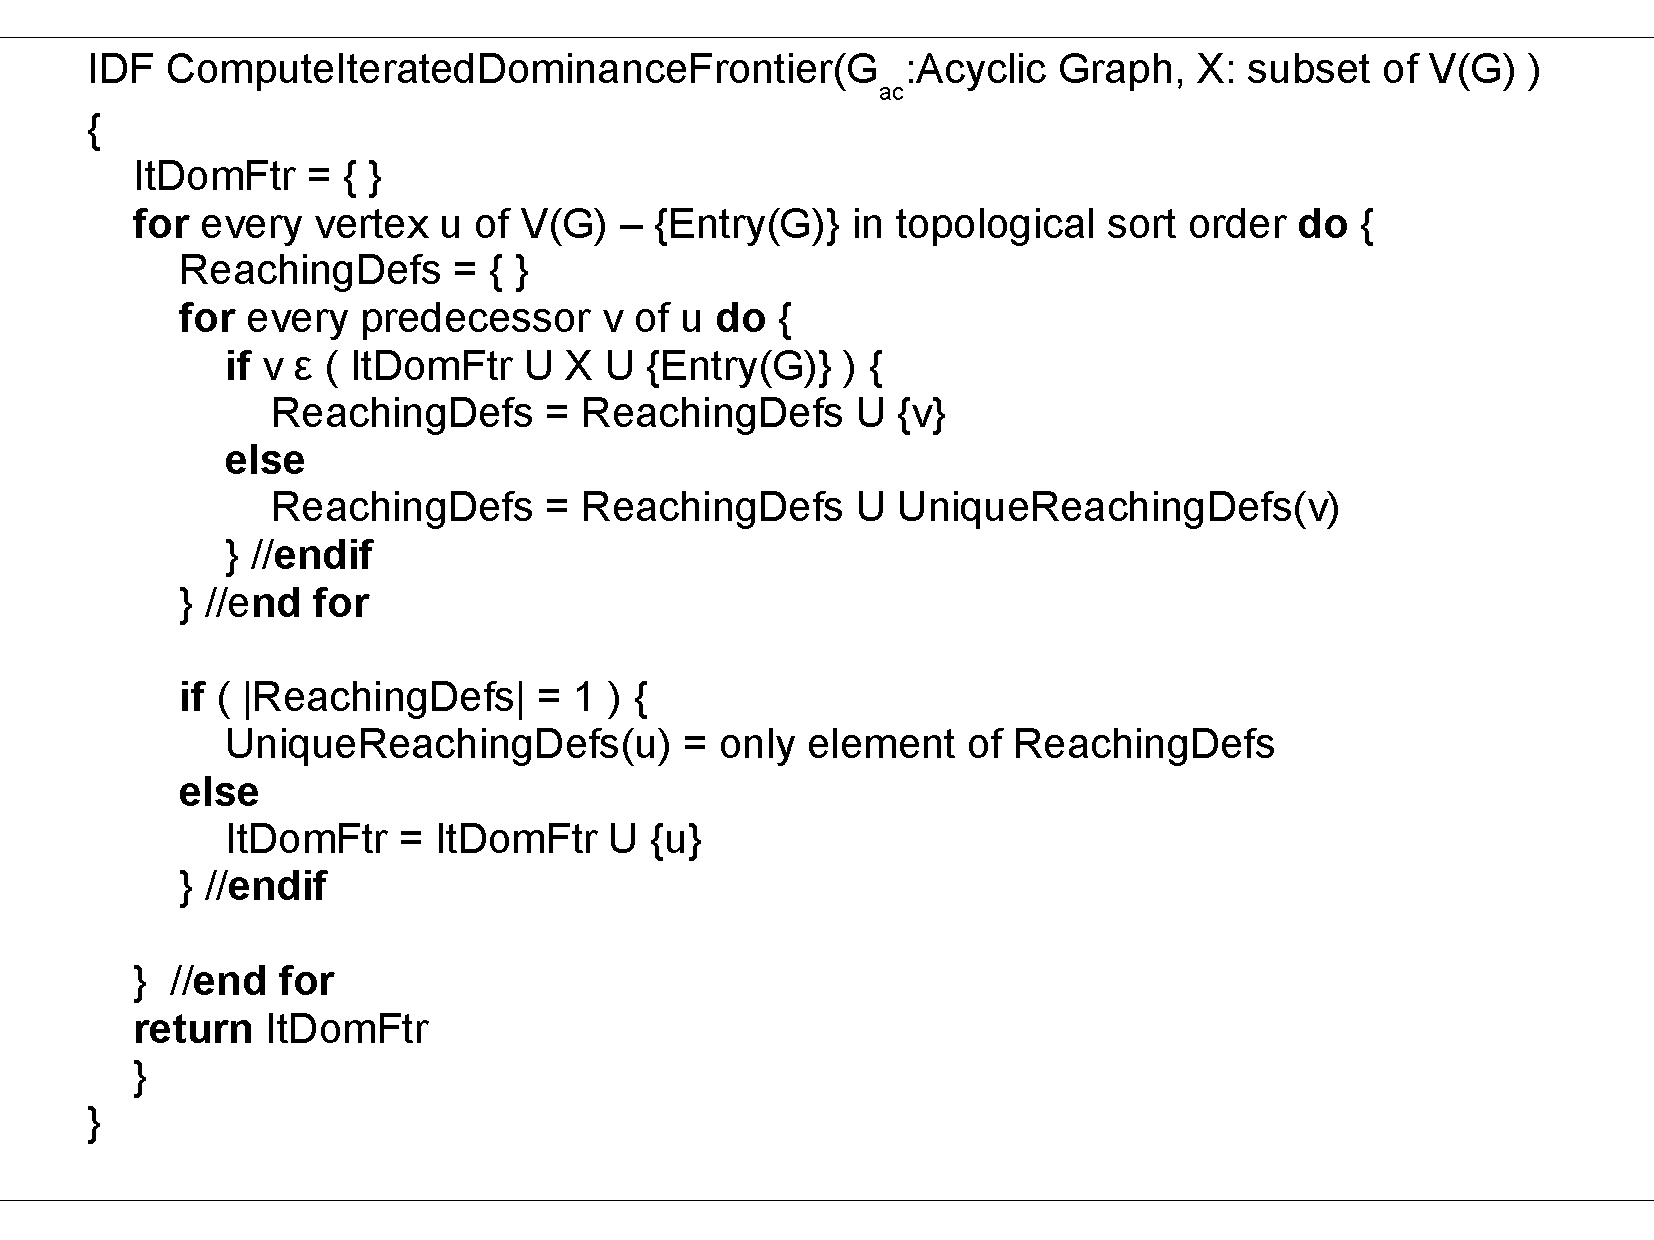
\includegraphics[scale=0.3]{idfcode.pdf}}
%\caption{Pseudocode for computing \iDF of an acyclic graph }
%\label{fig:idfcode}
%\end{figure}  

\begin{algorithm}
  \KwIn{$G_{\textit{ac}}$: acyclic CFG}
  \KwIn{$X$: subset of nodes}
  \KwOut{$\iDF(X)$}
  \caption{%ComputeIteratedDominanceFrontier($G_{\textit{ac}}$, $X$)
  Ramalingam's algorithm for \iDF in an acyclic graph.}
  \label{algo:ramaIDF}

  $\iDF \gets \emptyset$\;
  \lForEach{node $n$}{
    $\textit{UniqueReachingDef}(n) \gets \{\textit{entry}\}$\;
  }
  \ForEach{node $u \neq \textit{entry}$ in topological order}{
    $\textit{ReachingDefs} \gets \emptyset$\; 
    \ForEach{$v$ predecessor of $u$}{
      \If{$v \in \iDF \cup X \cup \textit{entry}$}{
      $\textit{ReachingDefs} \gets \textit{ReachingDefs} \cup \{v\}$; \label{C:rdf}
      }
      \Else{
      $\textit{ReachingDefs} \gets \textit{ReachingDefs} \cup 
      \textit{UniqueReachingDef}(v)$; \label{C:urdf}
      }
    }
    \If{$|\textit{ReachingDefs}| = 1$}{  \label{C:onerd}
      $\textit{UniqueReachingDef}(u) \gets \textit{ReachingDefs}$; 
    }
    \Else{
      $\iDF \gets \iDF \cup \{u\}$; \label{C:ridf}
    }
  } 
  \Return{$\iDF$}   
\end{algorithm}

Let us walk through this algorithm computing \iDF for variable $v$, i.e., $X = \{4,5,7,12\}$. The 
nodes in Figure~\ref{fig:lnf} are already numbered in topological order. Nodes~1 to~5 
have only one predecessor, none of them being in $X$, so their 
\textit{UniqueReachingDef} stays \textit{entry}, and \iDF is still empty. For 
node~6, its two predecessor belong to $X$, hence $\textit{ReachingDefs} = 
\{4,5\}$, and 6 is added to \iDF. Nothing changes for 7, then for 8 its 
predecessors 6 and 7 are respectively in \iDF and $X$: they are added to 
\textit{ReachingDefs}, and 8 is then added to \iDF. Finally, for nodes 8 to 12, 
their \textit{UniqueReachingDef} will be updated to node~8, but this will not 
change \iDF anymore which will end up being $\{6,8\}$.

\paragraph{\iDF on reducible graphs}

{\def\HLC{\mbox{HLC}}
A reducible graph can be decomposed into an acyclic graph and a set of back 
edges. The contribution of back edges to the iterated dominance frontier can be 
identified by using the loop nesting forest. If a vertex $u$ is contained in a 
loop, then $\iDF(u)$ will contain the loop header. For any vertex $u$, let 
$\HLC(u)$ denote the set of loop headers of the loops containing $u$. Given a 
set of vertices $X$, it turns out that $\iDF(X) = \HLC(X) \cup 
\iDFac(X \cup 
\HLC(X))$ where $\iDFac$ denote the \iDF restricted to the 
acyclic graph $G_{\textit{ac}}$.

Reverting back 
to Figure~\ref{fig:lnf}, we see that in order to find the $\iDF$ for the nodes 
defining $v$, we need to evaluate $\iDFac(\{4,5,7,12\} \cup 
\HLC(\{4,5,7,12\}))$. As all these nodes are contained in a single loop with 
header $2$ $\HLC(\{4,5,7,12\}) = \{2\}$.
Computing $\iDF\!ac(\{2,4,5,7,12\})$ gives us $\{6,8\}$, and finally, 
$\iDF(\{4,5,7,12\}) = \HLC(\{4,5,7,12\}) \cup \{6,8\} = \{2,6,8\}$.  
}

\paragraph{\iDF on irreducible graphs}

%\noindent
\begin{figure}[t]
  \centerline{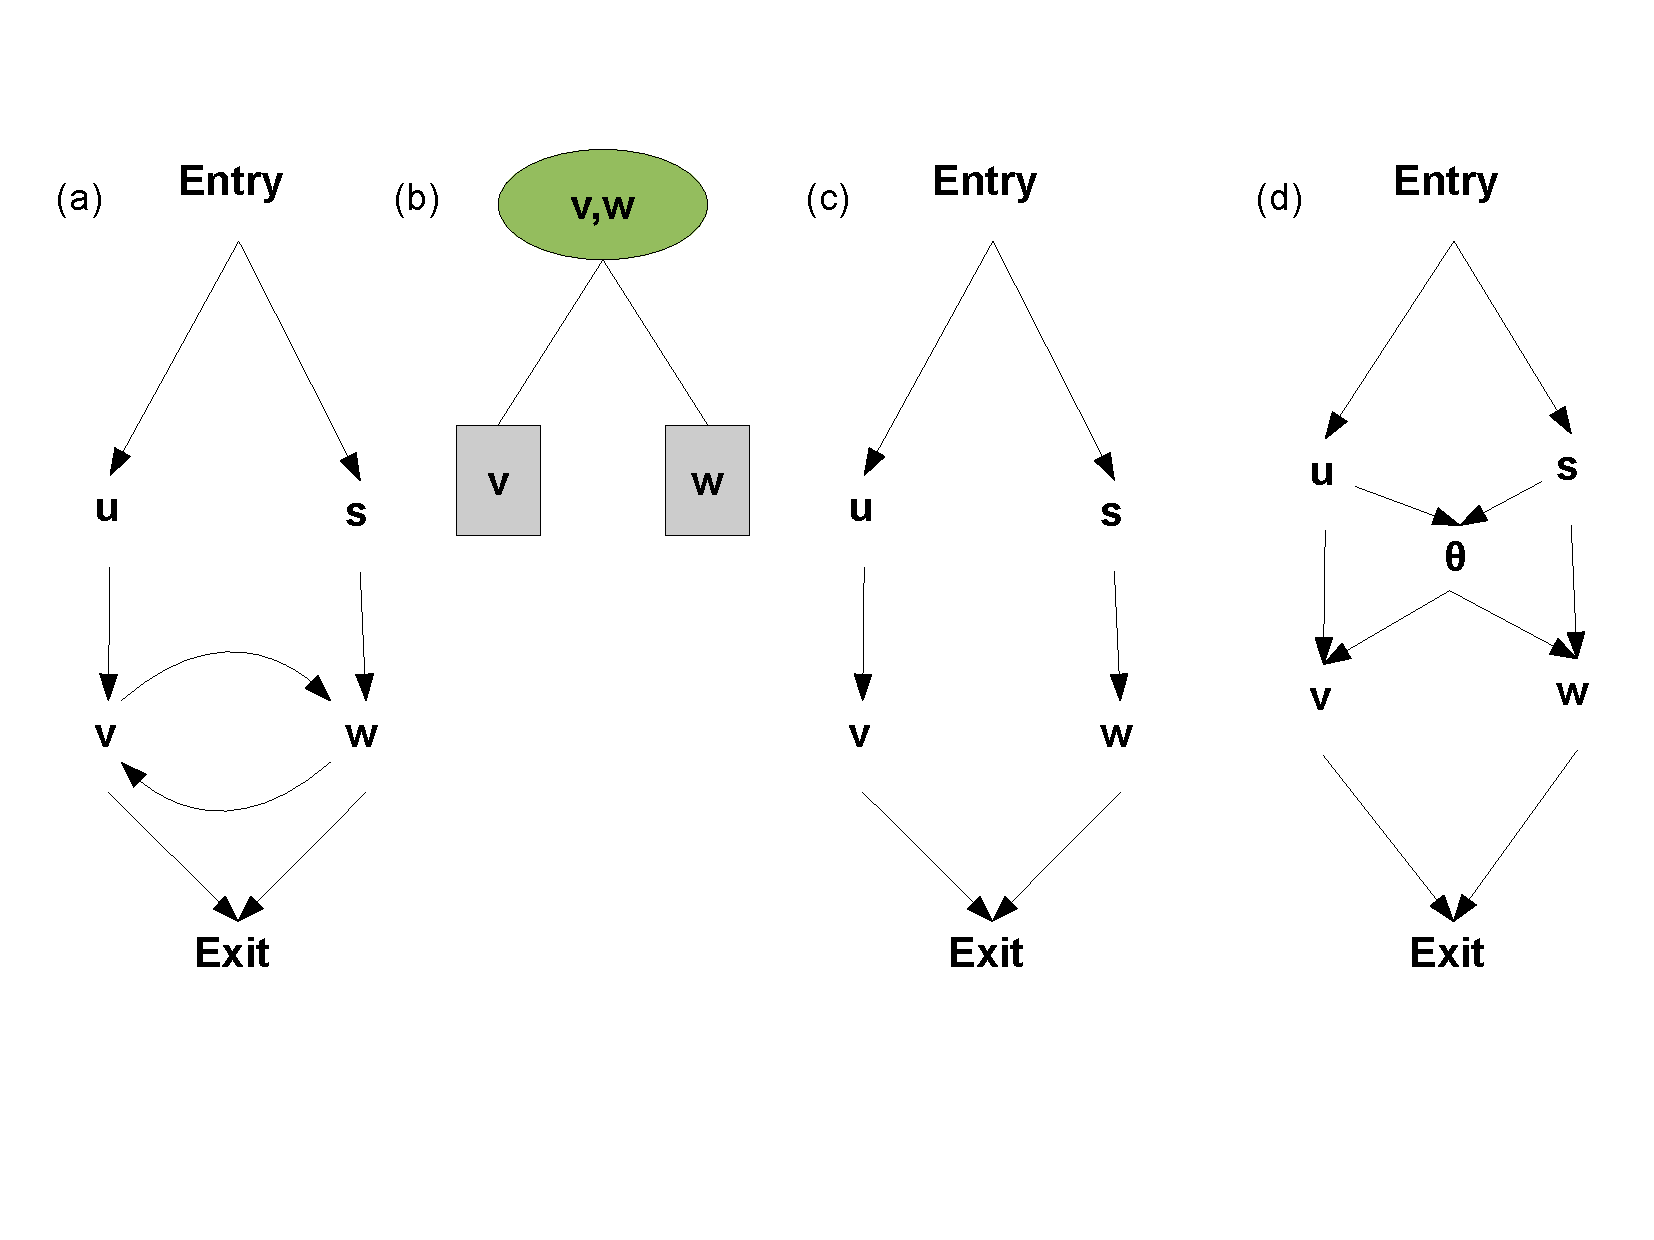
\includegraphics[scale=0.3]{irred.pdf}}
  \caption{(a) An irreducible graph (b) The Loop Nesting Forest (c) The acyclic subgraph (c) Transformed
  graph.}
  \label{fig:irred}
\end{figure} 



We will now briefly explain how graphs containing irreducible loops can be 
handled. The insight behind the implementation is to transform the irreducible 
loop in such a way that an acyclic graph is created from the loop without 
changing the dominance properties of the nodes.

\todo{subfigure}
The loop in the graph of Figure~\ref{fig:irred}(a) is irreducible as it has two 
headers, $v$ and $w$.
It can be transformed to the acyclic graph (c) by removing 
the edges between nodes $v$ and $w$ that create the irreducible loop.
We create a dummy node, $\theta$, to which we connect all predecessors of the 
headers ($u$ and $s$), and that we connect to all the headers of the loop 
($v$ and $w$), creating graph (d).

Following this transformation, the graph is now acyclic, and
computing the \iDF for the nodes in the original 
irreducible graph translates to computing \iDF using the transformed graph to 
get $\iDFac$ and using the loop forest of the original graph (b).

The 
crucial observation that allows this transformation to create an equivalent 
acyclic graph is the fact that the dominator tree of the transformed graph 
remains identical to the original graph containing an irreducible cycle. One of 
the drawbacks of the transformation is the possible explosion in the number of 
dummy nodes and edges for graphs with many irreducible cycles as a unique dummy 
node needs to be created for each irreducible loop.


\section{Concluding Remarks}

Although all these algorithms claim to be better than the original algorithm by Cyton et al., they are difficult to compare due to the unavailability of these algorithms in a common compiler framework. 

In particular, while constructing the whole \iDF set seems very costly in the classical construction algorithm, its cost is actually amortized as it will serve to place \phifuns for many variables.
It is however interesting not to pay this cost whenever we only have a few variables to consider, for instance when repairing SSA as in the next chapter.
 
Note also that people have observed in production compilers that, during SSA construction, what seems to be the most expensive part is the renaming of the variables and not the placement of \phifuns.



\section{Further Reading}

Cytron's approach for $\phi$-placement involves a fully eager approach of constructing the entire \DF-graph. On the other hand Sreedhar and Gao's approach is a fully lazy approach as it constructs \DF on-the-fly only when a query is encountered.
Pingali and Bilardi \cite{bilardi} suggested a middle-ground by combining both 
approaches. They proposed a new representation called ADT (Augmented Dominator 
Tree). The ADT representation can be thought as a \DJ-graph, where the \DF sets 
are pre-computed for certain nodes called ``boundary nodes'' using an eager 
approach. For the rest of the nodes, termed ``interior nodes,'' the \DF needs 
to be computed on-the-fly as in the Sreedhar-Gao algorithm. The nodes which act 
as ``boundary nodes'' are detected in a separate pass. A factor $\beta$ is used 
to determine the partitioning of the nodes of a CFG into boundary or interior 
nodes by dividing the CFG into zones. $\beta$ is a number that represents 
space/query-time tradeoff. $\beta <\!\!< 1$ denotes a fully eager approach where 
storage requirement for \DF is maximum but query-time is faster while 
$\beta >\!\!> 1$ denotes a fully lazy approach where storage requirement is zero but 
query is 
slower. 

Given the ADT of a control-flow graph, it is straight forward to 
modify  Sreedhar and Gao's algorithm for computing $\phi$-functions in linear time. The only modification that is needed is to ensure that we need not visit all the nodes of a sub-tree rooted at a node $y$ when $y$ is a boundary node whose \DF set is already known. This change is reflected in Line \ref{C:cached} of Figure~\ref{F:IDFMain}, where a subtree rooted at $y$ is visited or not visited based on whether it is a boundary node or not.

For iterative merge set computation, TDMSC-II is an improvement to algorithm 
TDMSC-I. This improvement is fueled by the observation that for an inconsistent 
node $u$, the merge sets of all nodes $w$ such that $w$ dominates $u$ and 
$w.\level \geq u.\level$,
can be locally corrected for some special cases. This
heuristic works very well for certain class of problems---especially for CFGs with \DF-graphs having cycles consisting of a few edges. This eliminates extra passes as an inconsistent node is made consistent immediately on being detected. For details of this algorithm refer to \cite{das}.


\paragraph{TODO: citations}
\begin{itemize}
  \item SSA form \cite{cfr}
  \item Sreedhar \& gao \cite{sreedhar_popl}
  \item Das \& Ramakrishna no explicit \DF-graph construction  \cite{das}
  \item Ramalingam loop nesting forest  \cite{rama}
  \item computing \iDF set without full \DF set \cite{sreedhar_popl,sreedharthesis}
  \item \cite{bilardi} 
\end{itemize}
}
